\documentclass{article}
\usepackage{fullpage}
\usepackage{color}
\usepackage[normalem]{ulem}
\newcommand{\eric}{\textcolor{blue}{[Eric]}}
\newcommand{\richard}{\textcolor{red}{[Richard]}}
\newcommand{\taylor}{\textcolor{green}{[Taylor]}}
\newcommand{\susi}{\textcolor{cyan}{[Susi]}}
\hyphenpenalty=100000
\usepackage{graphicx}
\DeclareGraphicsExtensions{.pdf,.png,.jpg}
\begin{document}
\setlength{\voffset}{3.5in}
\title{Milestone 3}
\author{Team Sriram\\
CM 1394\\
(Susi Cisneros, Eric Henderson, Taylor Purviance and Richard Thai)}
\date{13 January 2012}
\maketitle
\clearpage
\setlength{\voffset}{0pt}
\section{System Sequence Diagrams}
The system sequence diagrams show how the user and the system interact during the main operations of the system.
\subsection{Legend}
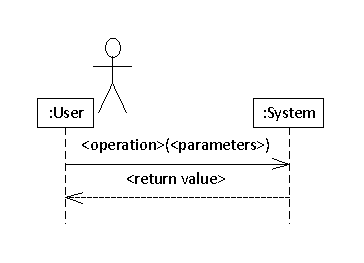
\includegraphics[keepaspectratio, width=6in]{ssd_legend.pdf}\\

\subsection{Add Item}
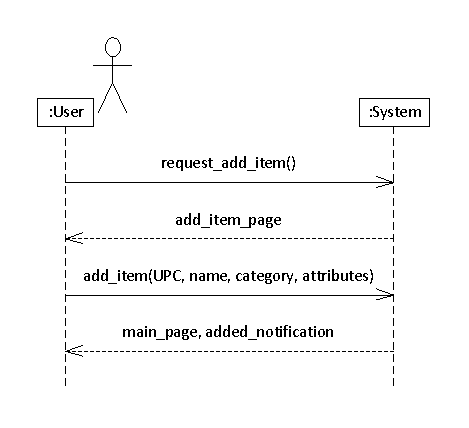
\includegraphics[keepaspectratio, width=6in]{ssd_add_item.pdf}\\

\subsection{View Item}
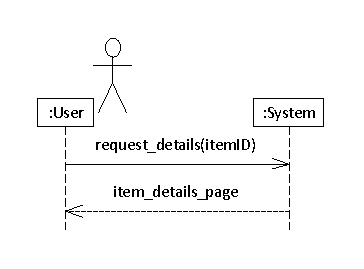
\includegraphics[keepaspectratio, width=6in]{ssd_view_item_details.pdf}\\

\subsection{Edit Item}
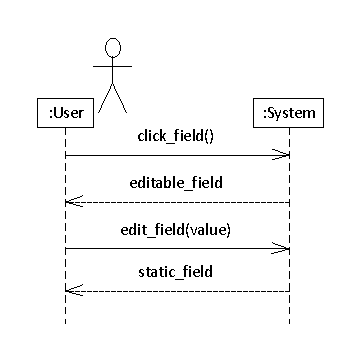
\includegraphics[keepaspectratio, width=6in]{ssd_edit_item_details.pdf}\\

\subsection{Basic Search}
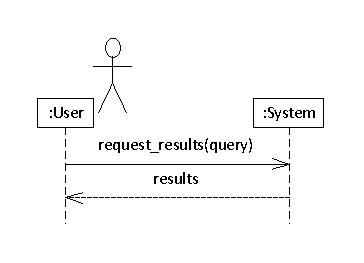
\includegraphics[keepaspectratio, width=6in]{ssd_basic_search.pdf}\\

\subsection{Advanced Search}
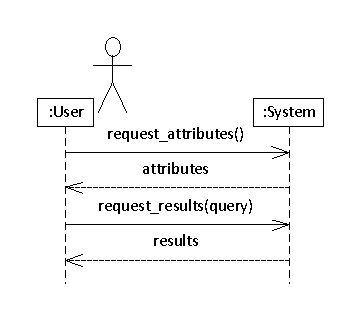
\includegraphics[keepaspectratio, width=6in]{ssd_advanced_search.pdf}\\

\subsection{Search Results Sorting}
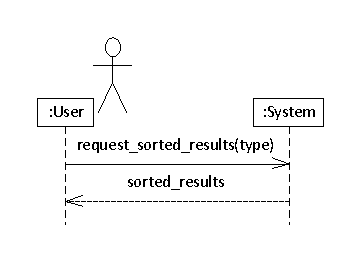
\includegraphics[keepaspectratio, width=6in]{ssd_search_result_sorting.pdf}\\

\subsection{Generate Report}
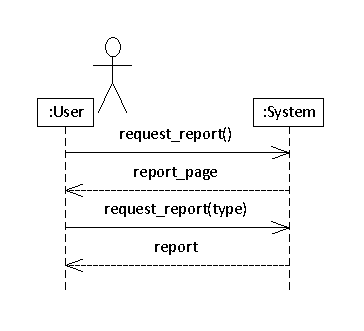
\includegraphics[keepaspectratio, width=6in]{ssd_generate_report.pdf}\\

\section{Operation Contracts}
The operation contracts show the difference between the state of the system before and after a command.  We choose to show the add item and edit field methods since the system sequence diagrams were not able to provide adequate detail for these operations.

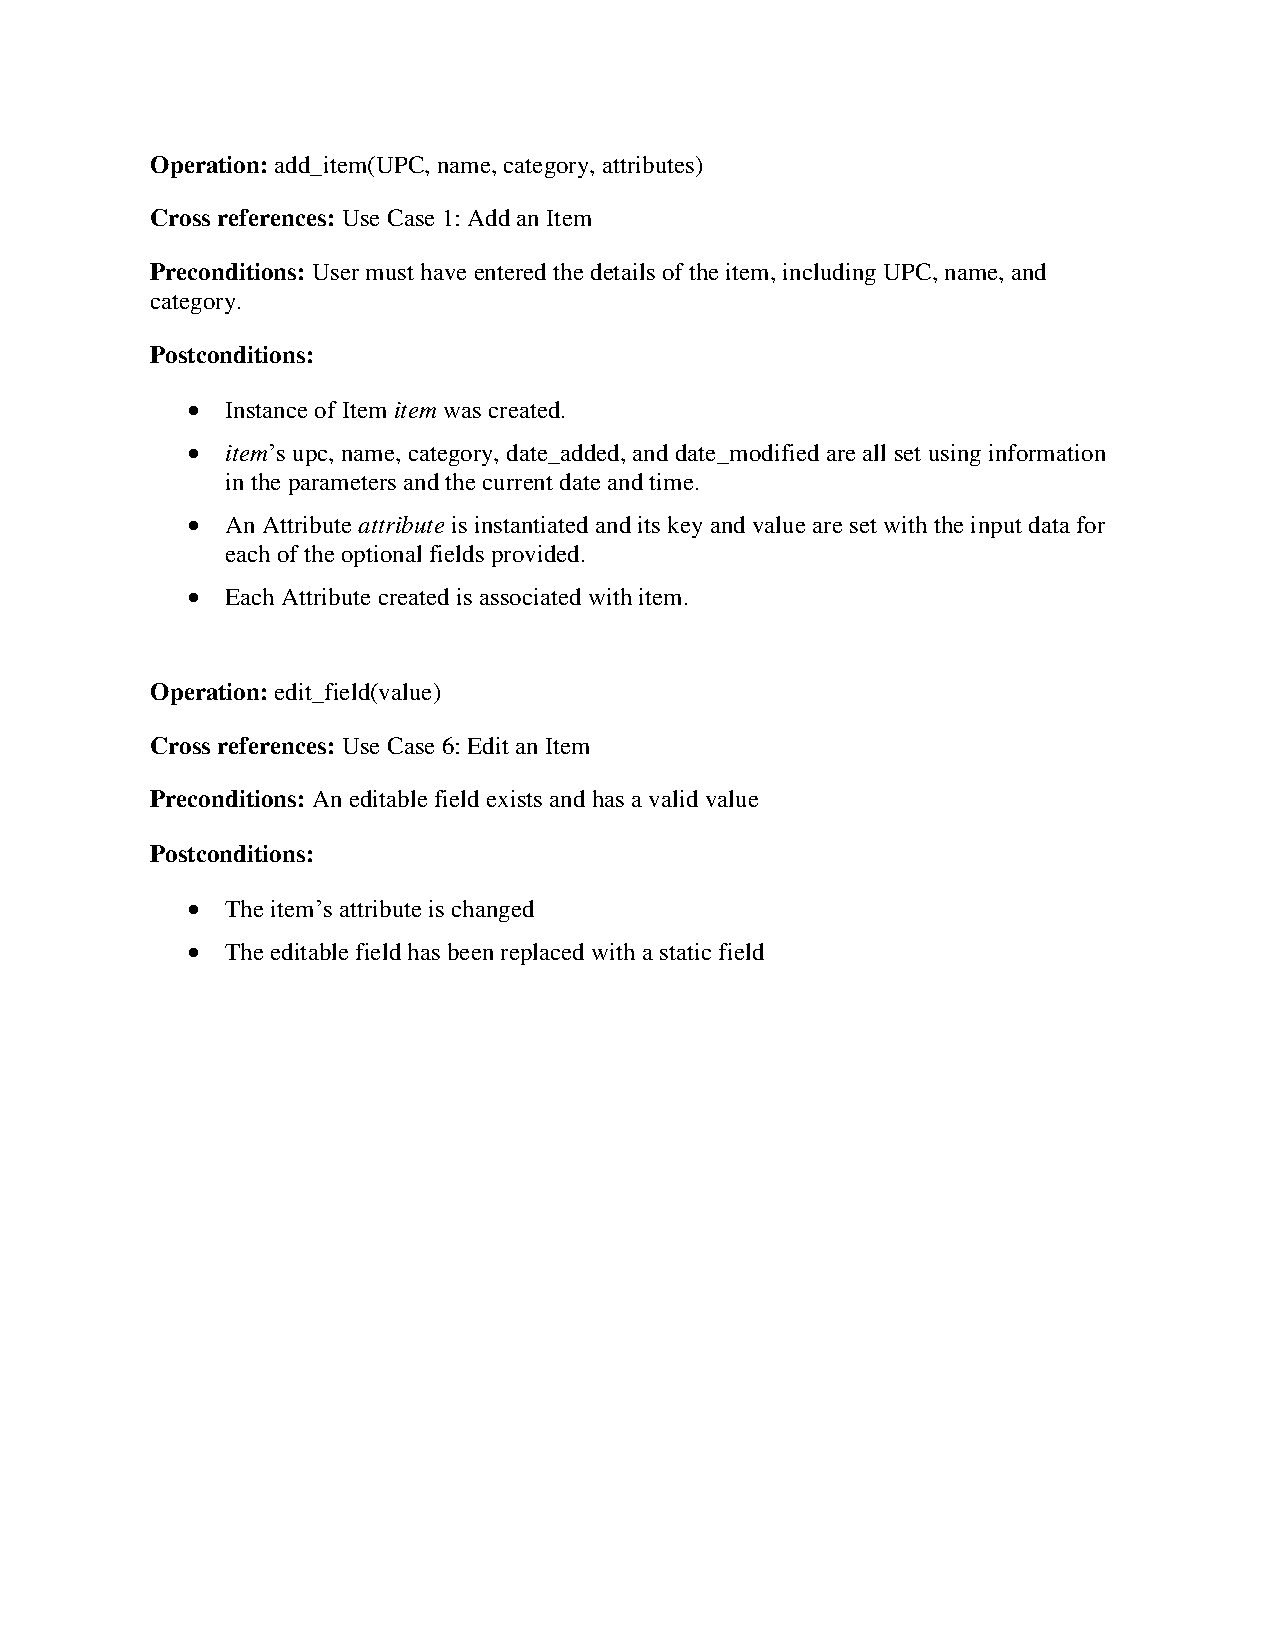
\includegraphics[keepaspectratio, width=6in]{Operational_Contracts.pdf}\\

\section{Logical Architecture and Package Diagram}
This diagram shows how the main elements of the system interact with each other.  It also shows which classes are part of the same layer.  The layers represent the three major parts of the system, the user interface, the domain of the system and the technical services that the system employs. 

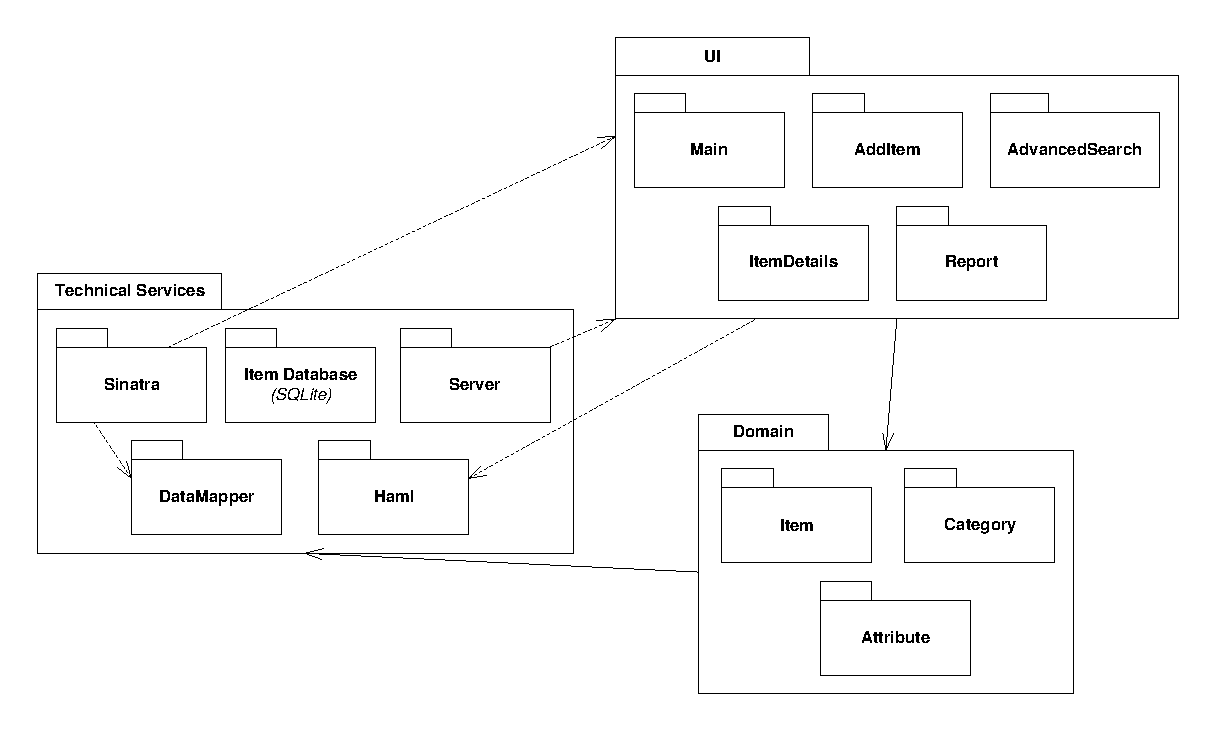
\includegraphics[keepaspectratio, width=6in]{package_diagram.pdf}\\

\section{Design Class Diagram}
The design class diagram shows the relationships the classes in the system have with each other.  It also shows the attributes each class has and the operations that each class can perform.

\subsection{Legend}
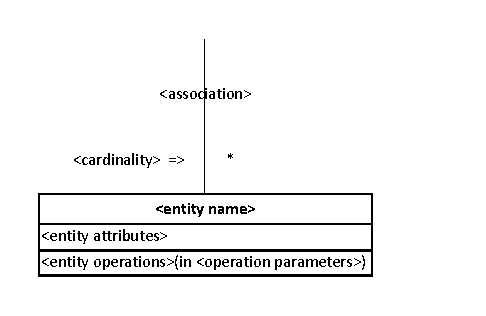
\includegraphics[keepaspectratio, width=6in]{class_diagram_legend.pdf}\\

\subsection{Diagram}
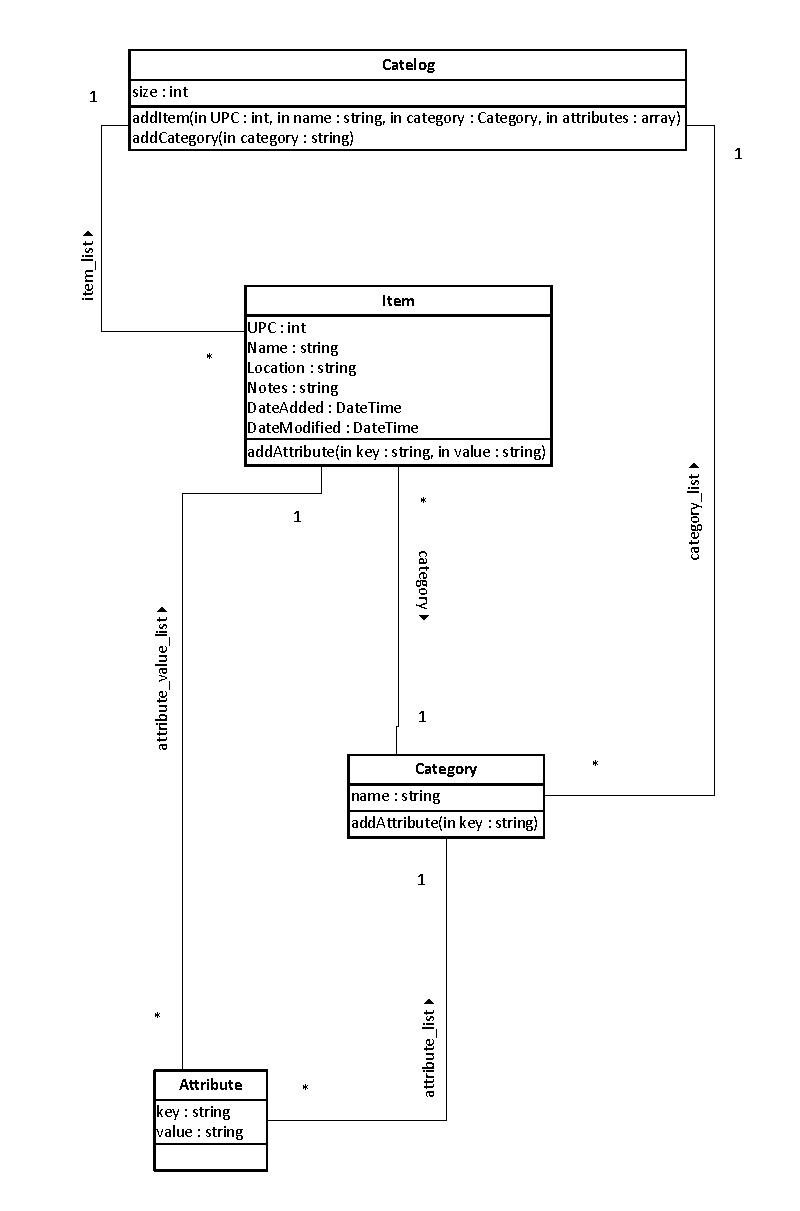
\includegraphics[keepaspectratio, width=6in]{class_diagram.pdf}\\

\section{Interaction Diagrams}
Interaction diagrams show how objects interact through messages.  For this system, we decided that sequence diagrams were more appropriate as they clearly communicate the order in which each action is performed.

\subsection{Sequence Diagrams}
\subsubsection{Legend}
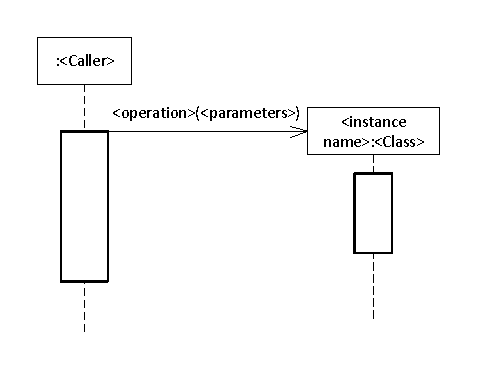
\includegraphics[keepaspectratio, width=6in]{sd_legend.pdf}\\

\subsubsection{Add Attribute to an Item}
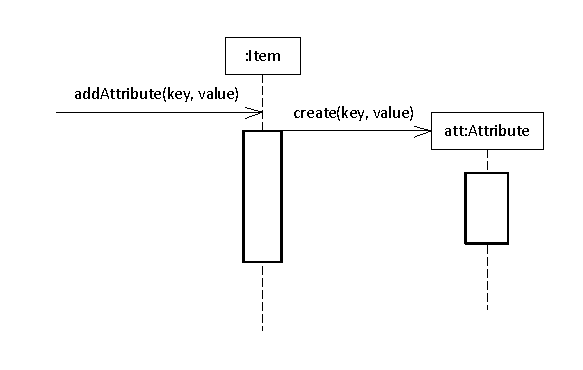
\includegraphics[keepaspectratio, width=6in]{sd_item_add_attribute.pdf}\\

\subsubsection{Add Item to the Catalog}
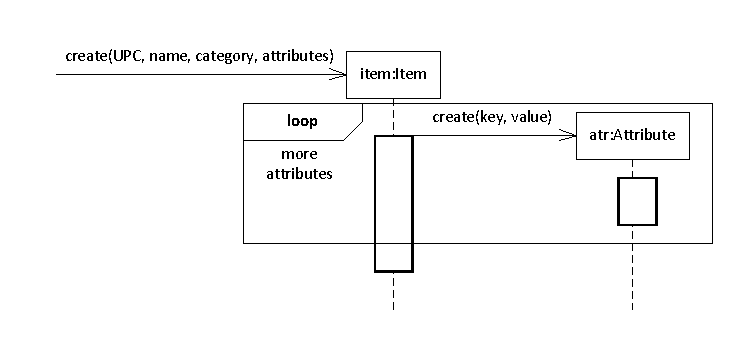
\includegraphics[keepaspectratio, width=6in]{sd_catalog_add_item.pdf}\\

\subsubsection{Add Category to the Catalog}
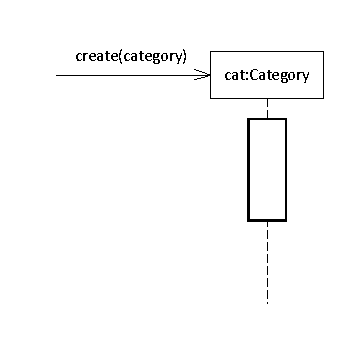
\includegraphics[keepaspectratio, width=6in]{sd_catalog_add_category.pdf}\\

\subsubsection{Add Attribute to the Category}
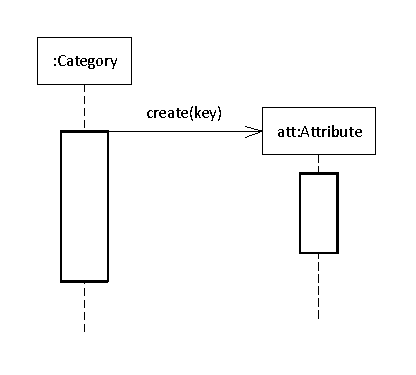
\includegraphics[keepaspectratio, width=6in]{sd_category_add_attribute.pdf}\\

\section{Who Done What Table}
\begin{tabular}{ | l | p{3in} | c | }
\hline
Team Member Names & Task/Comments & \# of hours effort\\
\hline
\hline
Richard Thai & Created SSDs, OCs, Package Diagram, DCD, SDs, Organized Meetings with PM and Client, Created web interfaces & 7\\
\hline
Eric Henderson & Created SSDs, OCs, Package Diagram, DCD, SDs, Created Visio Diagrams, Created DataMapper classes & 9\\
\hline
Susi Cisneros & Created SSDs, OCs, Package Diagram, DCD, SDs, Created DataMapper classes & 6\\
\hline
Taylor Purviance & Created SSDs, OCs, Package Diagram, DCD, SDs, Created web interfaces & 6\\
\hline
 &  & 28\\
\hline
\end{tabular}

\end{document}